\documentclass[runningheads]{llncs}

\usepackage[T1]{fontenc}
\usepackage[utf8]{inputenc}
\usepackage{graphicx}
\usepackage{booktabs}
\usepackage{amsmath}
\usepackage{amssymb}
\usepackage{cite}
\usepackage[hidelinks]{hyperref}

\setcounter{topnumber}{2}
\setcounter{bottomnumber}{1}
\setcounter{totalnumber}{3}
\renewcommand{\topfraction}{0.92}
\renewcommand{\bottomfraction}{0.55}
\renewcommand{\textfraction}{0.07}
\renewcommand{\floatpagefraction}{0.78}

\makeatletter
\setlength{\@fptop}{0pt}
\setlength{\@fpsep}{10pt plus 1fil}
\setlength{\@fpbot}{0pt plus 2fil}
\makeatother

% Sinh boi runners/make_paper3_tables.py -- dung sua tay.
% Prose KHONG duoc viet so truc tiep; dung macro o day.
\newcommand{\pdegFloor}{0.8504}
\newcommand{\pdegFloorFull}{0.8504201680672269}
\newcommand{\pqBestNonDeg}{0.8497}
\newcommand{\pselectedC}{0.01}
\newcommand{\pcGrid}{0.01, 0.1, 1, 10, 100}
\newcommand{\pcvFolds}{5}
\newcommand{\pcvScoring}{f1}
\newcommand{\pdegRecall}{1.000}
\newcommand{\pdegRecallStd}{0}
\newcommand{\pdegPrecision}{0.634}
\newcommand{\pdegTN}{0.0}
\newcommand{\pneuRecall}{0.943}
\newcommand{\pneuPrecision}{0.695}
\newcommand{\pneuTN}{9.8}
\newcommand{\pneuFone}{0.7977}
\newcommand{\pdegFone}{0.7760}
\newcommand{\pktaShared}{0.193395}
\newcommand{\pktaSharedFull}{0.19339506621329136}
\newcommand{\pperturbRangeOld}{0.000}
\newcommand{\pperturbRangeNew}{0.0194}
\newcommand{\pkPlateauFone}{0.8107}
\newcommand{\pkPlateauFrom}{80}
\newcommand{\pkSweepRuns}{35}
\newcommand{\pkSweepDeg}{0}
\newcommand{\prevRowsScanned}{840}
\newcommand{\prevModels}{7}
\newcommand{\prevDegRows}{9}
\newcommand{\prevDegModel}{SVM-RBF}
\newcommand{\prevQsvmMinRecall}{0.541}
\newcommand{\plegacyQubits}{4}
\newcommand{\plegacyN}{100}
\newcommand{\plegacySeeds}{5}
\newcommand{\prevQubits}{6}
\newcommand{\prevMaxN}{10\,000}
\newcommand{\prevRuns}{10}
\newcommand{\pcurveNc}{21}
\newcommand{\pcurveCmin}{0.001}
\newcommand{\pcurveCmax}{100}
\newcommand{\pcurveRuns}{5}
\newcommand{\pcurveEscapeC}{0.562341}
\newcommand{\pcurveFoneLo}{0.7760}
\newcommand{\pcurveFoneHi}{0.7978}
\newcommand{\pcurveFoneRise}{+0.0218}
\newcommand{\pcurveMacroLo}{0.3880}
\newcommand{\pcurveMacroHi}{0.5627}
\newcommand{\pcurveMacroRise}{+0.1747}
\newcommand{\pcurveRiseRatio}{8}
\newcommand{\preproCv}{0}
\newcommand{\preproTest}{2.2e-16}
\newcommand{\pobjQBinC}{0.562}
\newcommand{\pobjQBinDeg}{0/5}
\newcommand{\pobjQMacC}{10}
\newcommand{\pobjQMacDeg}{0/5}
\newcommand{\pobjQBalC}{10}
\newcommand{\pobjQBalDeg}{0/5}
\newcommand{\pobjLinBinC}{0.0562}
\newcommand{\pobjLinBinDeg}{1/5}
\newcommand{\pobjLinMacC}{0.0562}
\newcommand{\pobjLinMacDeg}{1/5}
\newcommand{\pobjLinBalC}{0.0562}
\newcommand{\pobjLinBalDeg}{1/5}
\newcommand{\pobjRbfBinC}{0.316}
\newcommand{\pobjRbfBinDeg}{1/5}
\newcommand{\pobjRbfMacC}{31.6}
\newcommand{\pobjRbfMacDeg}{0/5}
\newcommand{\pobjRbfBalC}{31.6}
\newcommand{\pobjRbfBalDeg}{0/5}
\newcommand{\pcurveEvals}{420}
\newcommand{\pcurveTnZeroFnPos}{0}
\newcommand{\pfloorFoldStd}{0.015}
\newcommand{\pbestNonDegFoldStd}{0.055}
\newcommand{\pfloorGap}{0.0007}
\newcommand{\pkSelect}{35}
\newcommand{\ptrainAttackRatio}{0.74}
\newcommand{\ptestAttackRatio}{0.634}
\newcommand{\pnFiveHundredTrainRatio}{0.74}
\newcommand{\pperturbSigmas}{0.05, 0.1, 0.2}
\newcommand{\pprQHundred}{2}
\newcommand{\pprLinHundred}{1}
\newcommand{\pprMaxFiveHundred}{0}
\newcommand{\pprOneSeLinFive}{1}
\newcommand{\pprOneSePolyFive}{2}
\newcommand{\pprBalQFive}{1}
\newcommand{\pnFiveBaseline}{0.848}
\newcommand{\pnFiveFoldStdMax}{0.034}
\newcommand{\pmacroHundredLo}{0.55}
\newcommand{\pmacroHundredHi}{0.59}
\newcommand{\pmacroFiveLo}{0.60}
\newcommand{\pmacroFiveHi}{0.71}
\newcommand{\pedgeQ}{0.1}
\newcommand{\pedgeRbf}{0.1}
\newcommand{\pedgeLin}{0.018}
\newcommand{\pedgePoly}{0.0056}
\newcommand{\pspreadQ}{0.27}
\newcommand{\pspreadRbf}{0.36}
\newcommand{\pspreadLin}{4.6}
\newcommand{\pspreadPoly}{5.3}
\newcommand{\prevRbfC}{0.1}
\newcommand{\prevTuneN}{2\,000}
\newcommand{\pnLarge}{500}


\newcommand{\QSVM}{QSVM}
\newcommand{\ZZ}{\textsf{ZZ}}
\newcommand{\Fone}{F_1}
\newcommand{\fundingcode}{T2026-02-10TN}

\begin{document}

\title{When Model Selection Manufactures a Finding: A Tuning Trap in
Quantum-Kernel Intrusion Detection}

  \author{Quan Tran Anh Vo \and
          Minh Tuan Pham\thanks{Corresponding author: pmtuan@dut.udn.vn} \and
          Quang Anh Nguyen \and
          Nguyen Nang Hung Van}
  \authorrunning{Q. T. A. Vo et al.}
  \titlerunning{A Tuning Trap in Quantum-Kernel IDS}
  \institute{University of Science and Technology -- The University of
    Danang, Da Nang, Vietnam}

\maketitle

\begin{abstract}
Selecting a hyper-parameter by cross-validated binary $\Fone$ on
class-imbalanced data can return a model that assigns every record to one
class. We document a case in which this happened to a four-qubit
quantum-kernel intrusion detector on UNSW-NB15: the selected model produced an
apparent robustness result, refuted only when the regularisation constant was
held fixed. The constant all-attack classifier scores a high binary $\Fone$,
and on a small sample no point of a coarse grid beat it by more than
fold-to-fold noise. A census shows that the collapse is not specific to the
quantum kernel, although the kernel's scale decides where on the $C$ axis it
occurs. We then measure the standard remedies. Macro $\Fone$, MCC and a
minority-positive $\Fone$ avoided collapse whenever $C$ was selected on the
run it was applied to, while even a class-averaged objective could collapse
when $C$ was transferred from another run; a denser grid, class weighting and the one-standard-error rule
each failed at least once, and a larger sample removed the trap for
$\arg\max$ but not for the one-standard-error rule. The check that identified every case is the count of predicted
negatives, and we release the checks that implement it.
\keywords{Quantum kernel \and Model selection \and Class imbalance \and
Intrusion detection \and Reproducibility}
\end{abstract}

\section{Introduction}\label{sec:intro}

Quantum-kernel classifiers~\cite{havlicek2019,schuld2019hilbert} have been
applied to intrusion
detection~\cite{payares2021dos,kalinin2023qids,abreu2025quantumnetsec,kaissar2026survey}.
Evaluating any such classifier requires choosing a regularisation constant
$C$, usually by maximising a cross-validated score. On class-imbalanced data
that procedure has a trap. The constant classifier that calls everything an
attack attains a respectable binary $\Fone$, and a model whose genuine scores
do not clearly exceed it can have the degenerate setting returned to it by
$\arg\max$. Each ingredient is known: $\Fone$ ignores true
negatives~\cite{chicco2020mcc}, a small $C$ yields the majority
class~\cite{cortes1995svm}, and selection over-fits the validation
data~\cite{cawley2010overfitting}. What this paper contributes is a measured
account of how they combined in a real study, which remedies would have caught
it, and where the kernel enters.

The case occurred for a four-qubit quantum-kernel detector in our own earlier
work~\cite{companion} on UNSW-NB15~\cite{moustafa2015unsw}.

The selected model predicted the attack class for every test record and went
on to produce a robustness result --- $\Fone$ invariant under input noise ---
that was an artefact of the constant prediction. It was caught only when $C$
was fixed at a neutral value and the experiment re-run.

\paragraph{Contributions.}
\begin{enumerate}
  \item A documented case in which $\arg\max$ selection over a
        cross-validated binary-$\Fone$ grid returned a degenerate classifier
        that then produced an apparent robustness result
        (Sections~\ref{sec:trap}--\ref{sec:kernel}).
  \item The mechanism and its fragility: the quantum kernel's best
        non-degenerate score fell short of the constant classifier's by
        \pfloorGap, far inside the fold-to-fold standard deviation
        (Section~\ref{sec:trap}).
  \item A census and a per-run re-selection showing that the collapse is not
        specific to the quantum kernel, while the kernel's scale sets where on
        the $C$ axis it occurs (Section~\ref{sec:census}).
  \item Measured remedies at two sample sizes (Section~\ref{sec:catch},
        Tables~\ref{tab:objective} and~\ref{tab:remedies}).
  \item Audit checks that detect the failure, released with the paper
        (Section~\ref{sec:checks}).
\end{enumerate}

\section{Related work}\label{sec:related}

\paragraph{Quantum kernels and intrusion detection.}
Quantum feature maps were proposed as kernels that are hard to evaluate
classically~\cite{havlicek2019,schuld2019hilbert}, and a separation was
established for a constructed learning problem~\cite{liu2021speedup}. Later
work showed that any advantage also depends on the data~\cite{huang2021power},
that the bandwidth of a quantum kernel governs whether it
generalises~\cite{shaydulin2022bandwidth}, and that fidelity kernels
concentrate towards a constant as the number of qubits
grows~\cite{thanasilp2024concentration}. Applied studies carried these kernels
to intrusion detection. Payares and Mart\'{\i}nez-Santos~\cite{payares2021dos}
compare a quantum SVM, a hybrid quantum--classical network and a two-processor
ensemble for DDoS detection on CIC-DDoS2019; Kalinin and
Krundyshev~\cite{kalinin2023qids} evaluate a quantum SVM and a quantum
convolutional network on their own packet data; Abreu
\emph{et al.}~\cite{abreu2025quantumnetsec} combine quantum and classical
stages on public IDS datasets; Kaissar \emph{et al.}~\cite{kaissar2026survey}
survey the area and the metrics it reports. The first two report confusion
matrices beside their aggregate scores, which is the practice this paper
argues for. Our concern is not with these studies, whose selection procedures
cannot be audited from the printed record, but with a failure that selection
can introduce before any reported number is computed.

\paragraph{Metrics and model selection under imbalance.}
That binary $\Fone$ flatters a classifier on imbalanced data is
established~\cite{he2009imbalanced,chicco2020mcc,christen2023fmeasure,saito2015prc}.
Chicco and Jurman~\cite{chicco2020mcc} argue for the Matthews correlation
coefficient (MCC) because it reads all four cells of the confusion matrix.
Forman and Scholz~\cite{forman2010apples} show that how $F$ is aggregated over
folds matters under imbalance: averaging per-fold scores is biased relative to
pooling the counts. Cawley and Talbot~\cite{cawley2010overfitting} show that
model selection itself over-fits the validation data. In computer security,
Arp \emph{et al.}~\cite{arp2022mlsec} list biased parameter selection,
inappropriate performance measures and the base-rate fallacy among ten
recurring pitfalls. The case below combines them: the flattering measure is
the \emph{selection} objective, so it does not misdescribe a model --- it
chooses one, and every downstream number then describes a constant classifier.

\paragraph{The constant $C$ and the degenerate solution.}
The soft-margin formulation~\cite{cortes1995svm} weighs margin width against
the summed hinge loss. As $C$ falls the margin term dominates, and on an
imbalanced sample the minimiser approaches the majority-class constant. That
is standard. The question here is when a selection objective prefers that
solution to every non-degenerate alternative on the grid.

\section{Setup}\label{sec:setup}

Both protocols use the same front end on UNSW-NB15: one-hot encoding,
\textsc{SelectKBest} with $K = \pkSelect$, PCA to as many components as
qubits, and a min--max map onto $[0,\pi]$. Every transformer is fitted on the
training split alone and, during cross-validation, refitted inside each
training fold, so validation folds never inform the features. The quantum
kernel is the \ZZ{}-FeatureMap with two repetitions and full entanglement,
evaluated as an exact statevector fidelity. Classical kernels are linear,
degree-two polynomial and RBF (bandwidth by scikit-learn's \texttt{scale}
rule), all fitted by the same soft-margin solver, so arms differ only in the
kernel and $C$. The attack class is positive unless stated otherwise.

The \emph{tuned} protocol uses \plegacyQubits{} qubits and \plegacySeeds{}
runs with $N_{\text{train}} = N_{\text{test}} = \plegacyN$, each drawn by
stratified sampling from disjoint partitions of the official training and test
files, with a minimum count for every rare attack category. Attacks form a
fraction \ptrainAttackRatio{} of each training split and \ptestAttackRatio{}
of each test split, on average. $C$ is chosen once, on the training split of run~1, by
$\arg\max$ of the mean of \pcvFolds{} stratified per-fold binary $\Fone$
scores over $\{\pcGrid\}$, ties going to the smaller $C$; that value is then
applied to every run. The earlier study's robustness experiment added Gaussian
noise with $\sigma \in \{\pperturbSigmas\}$ to the PCA features of the test
records before scaling, and reported the spread of $\Fone$ across $\sigma$.
The \emph{revision} protocol uses \prevQubits{} qubits, training sizes up to
$\prevMaxN$ and \prevRuns{} runs; in one of its arms the classical SVMs use a
$C$ tuned once on a separate stratified set of \prevTuneN{} records by macro $\Fone$ with the
one-standard-error (one-SE) rule. Every claim below states its protocol.

\section{The trap}\label{sec:trap}

\begin{figure}[t]
  \centering
  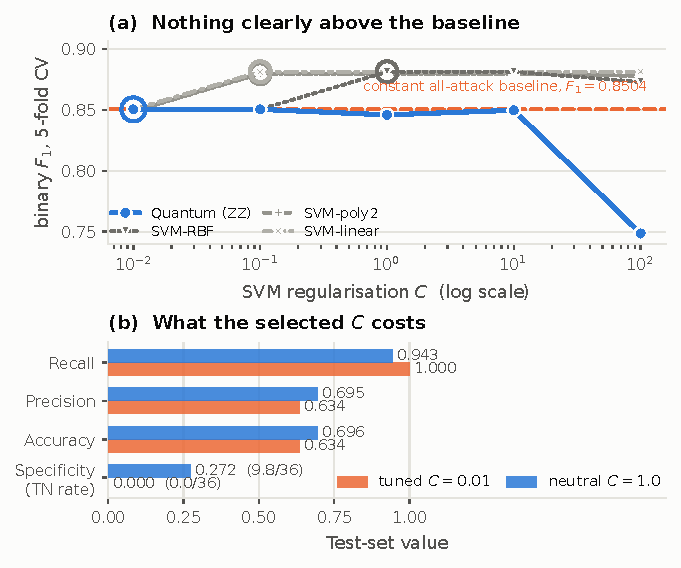
\includegraphics[width=\textwidth]{figs/fig1_tuning_trap.pdf}
  \caption{(a) Five-fold cross-validated binary $\Fone$ (attack positive) on
  the training split of run~1, against $C$. The dashed line is the score of
  the constant all-attack classifier on the same folds, $\pdegFloor$. All four
  kernels sit on it at $C = \pselectedC$; the linear and polynomial kernels
  rise above it at $C = 0.1$ and the RBF kernel at $C = 1$, while the quantum
  kernel's best non-degenerate score is $\pqBestNonDeg$. Circles mark what
  $\arg\max$ returns. (b) What that selection costs on the test set.}
  \label{fig:trap}
\end{figure}

We call a model degenerate on a run when it predicts the attack class for
every test record, i.e.\ $\mathrm{TN} = \mathrm{FN} = 0$, and we check this
directly on the predictions. Across all \pcurveEvals{} test evaluations of
Section~\ref{sec:catch}, \pcurveTnZeroFnPos{} had $\mathrm{TN} = 0$ with
$\mathrm{FN} > 0$, so in this study $\mathrm{TN} = 0$ alone would have given
the same counts.

On the tuned protocol the search returned $C = \pselectedC$ for the quantum
kernel. On the test set the selected model has recall $\pdegRecall$ on all
\plegacySeeds{} runs, precision $\pdegPrecision$ --- the attack fraction of
the test splits --- and $\mathrm{TN} = \pdegTN$.

Three $\Fone$ values recur below and must not be confused. The binary $\Fone$
of the constant classifier depends only on the attack fraction: it is
$\pdegFloor$ on the training folds of run~1 and $\pdegFone$ on the test
splits. Macro $\Fone$, which averages the two classes, gives the same
classifier $\pcurveMacroLo$ on the test splits.

The mechanism is Fig.~\ref{fig:trap}(a). Every kernel reaches the constant
baseline at $C = \pselectedC$. The linear and polynomial kernels climb above
it once $C \ge 0.1$, so $\arg\max$ moves away. The quantum kernel's best
non-degenerate grid score is $\pqBestNonDeg$, \pfloorGap{} below the baseline,
whereas the fold-to-fold standard deviations of the two scores are
\pfloorFoldStd{} and \pbestNonDegFoldStd. Selection therefore did not find the
degenerate model better; it could not tell the two apart, and the tie-breaking
towards small $C$ did the rest. The baseline is a score available on this
grid and these folds, not a universal floor: it moves with the attack
fraction, and false positives still lower it through precision. The grid also
matters. Its five points are a decade apart, and Section~\ref{sec:catch} shows
that the quantum kernel escapes collapse between two of them.

\section{The Gram matrix is not the cause}\label{sec:kernel}

\begin{figure}[t]
  \centering
  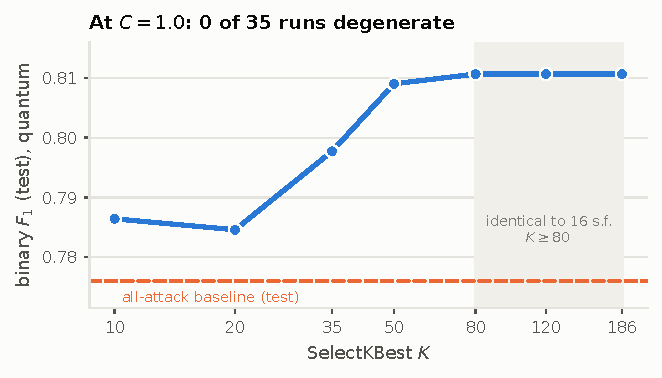
\includegraphics[width=\textwidth]{figs/fig2_k_sweep.pdf}
  \caption{With $C$ held at a neutral $1.0$, the quantum kernel is degenerate
  on \pkSweepDeg{} of \pkSweepRuns{} runs across seven \textsc{SelectKBest}
  budgets, and its binary test $\Fone$ plateaus at $\pkPlateauFone$ for
  $K \ge \pkPlateauFrom$. The dashed line is the binary test $\Fone$ of the
  all-attack classifier.}
  \label{fig:ksweep}
\end{figure}

Refitting the same cached Gram matrices with $C = 1.0$ raises recall to
$\pneuRecall$, precision to $\pneuPrecision$ and $\mathrm{TN}$ to $\pneuTN$,
and binary $\Fone$ from $\pdegFone$ to $\pneuFone$. The Gram matrices are
identical in both settings, so the collapse was produced by the choice of $C$
and not by a different kernel. That does not mean the kernel plays no part:
Section~\ref{sec:census} shows that its scale sets the value of $C$ at which
collapse occurs.

The apparent robustness result is visible in the same artifacts: the spread of
$\Fone$ across the three noise levels was $\pperturbRangeOld$ under the
selected $C$ --- invariant, because the prediction was constant --- against
$\pperturbRangeNew$ once $C$ was held fixed.

\section{A degeneracy census}\label{sec:census}

% Sinh boi runners/make_paper3_tables.py -- dung sua tay.
\begin{table}[t]
\centering
\caption{Degeneracy census. A model is degenerate on a run when it
predicts the attack class for every test record, i.e.\ $\mathrm{TN}
= \mathrm{FN} = 0$, checked directly on the predictions. Tuned rows
use the $C$ selected once on the training split of run~1. The
revision row is the RBF kernel at $N_{\text{train}} = 100$ with the
$C$ tuned once on a separate set; no other model, size or arm of
that protocol is degenerate.}
\label{tab:degeneracy}
\begin{tabular}{l@{\hskip 1.2em}l@{\hskip 1.4em}r@{\hskip 1.4em}r@{\hskip 1.2em}r}
\toprule
Protocol & Model & Selected $C$ & Degenerate & Runs \\
\midrule
tuned & Quantum (ZZ) & 0.01 & 5 & 5 \\
 & SVM-linear & 0.1 & 1 & 5 \\
 & SVM-poly2 & 0.1 & 1 & 5 \\
 & SVM-RBF & 1 & 0 & 5 \\
\addlinespace[2pt]
tuned data, neutral $C$ & Quantum (ZZ) & 1 & 0 & 35 \\
\addlinespace[2pt]
revision, $N=100$ & SVM-RBF & 0.1 & 9 & 10 \\
\bottomrule
\end{tabular}
\end{table}


Table~\ref{tab:degeneracy} counts, for each protocol and model, the runs on
which the fitted classifier is degenerate.

\paragraph{Collapse is not a quantum phenomenon.}
Under the tuned protocol it occurs for three of the four kernels. Re-selecting
$C$ separately on each run's own training split (Table~\ref{tab:remedies},
first row) gives \pprQHundred{} degenerate runs of five for the quantum kernel
and \pprLinHundred{} for each classical kernel, so the five-of-five count in
Table~\ref{tab:degeneracy} owes much to selecting once on run~1 and
transferring that $C$. Under the revision protocol, whose model set also
includes a random forest~\cite{breiman2001rf} and gradient-boosted
trees~\cite{chen2016xgboost}, a scan of \prevRowsScanned{} rows across
\prevModels{} models finds \prevDegRows{} degenerate rows, all belonging to
the RBF kernel at $N_{\text{train}} = \plegacyN$ and none to the quantum
kernel (whose lowest macro recall in that scan is \prevQsvmMinRecall).

Those rows have a simple cause. The tuned-once arm of the revision protocol
chose the classical $C$ on \prevTuneN{} records, where the one-SE rule chose $C = \prevRbfC$.
Because $C$ multiplies the \emph{summed} hinge loss, the same value
regularises far more strongly on \plegacyN{} training records, and there it
returned a constant classifier on \prevDegRows{} runs of \prevRuns; at every larger training
size it did not. A $C$ tuned at one sample size and reused at a much smaller
one is thus a second route into the trap.

\paragraph{Where the kernel enters.}
At $C = 1$ no run collapses for any kernel. Below that, the largest $C$ at
which every run collapses differs by kernel: \pedgePoly{} for the polynomial
kernel, \pedgeLin{} for the linear kernel, and \pedgeRbf{} for both the RBF
and the quantum kernel. The order follows the spread of the off-diagonal Gram
entries on the training split, whose standard deviations are \pspreadPoly,
\pspreadLin, \pspreadRbf{} and \pspreadQ{} respectively. With small $C$ every
dual coefficient is capped at $C$, so the part of the decision function that
varies between test records is bounded by $C$ times the variation of the
kernel entries, and the intercept, which favours the majority class, wins
until $C$ compensates. The fidelity kernel has the least spread, consistent
with the concentration of quantum kernels~\cite{thanasilp2024concentration},
and so needs a large $C$ to escape. At four qubits that concentration is mild,
and we report the ordering as an observed mechanism, not as proof that quantum
kernels are generally more exposed.

\paragraph{A neutral $C$ removes the effect.}
Holding $C = 1$ gives \pkSweepDeg{} degenerate runs out of \pkSweepRuns{}
(Fig.~\ref{fig:ksweep}). The revision rows of Table~\ref{tab:degeneracy}
are recomputed from runs the companion study~\cite{companion} reports, but
count a quantity it does not report, so the census is a new measurement over
existing runs.

\section{What would have caught it}\label{sec:catch}

We first reuse the stored Gram matrices of the tuned protocol, so no quantum
circuit is evaluated again. We refit at \pcurveNc{} values of $C$ spaced
logarithmically from \pcurveCmin{} to \pcurveCmax{} (the original five points
included) on all \pcurveRuns{} runs and repeat the selection under three
objectives. The same code path first reproduces the published numbers: the
cross-validated $\Fone$ at the original grid points agrees to \preproCv{}, and
the test-set means at the tuned and at the neutral $C$ agree to \preproTest.

\begin{figure}[t]
  \centering
  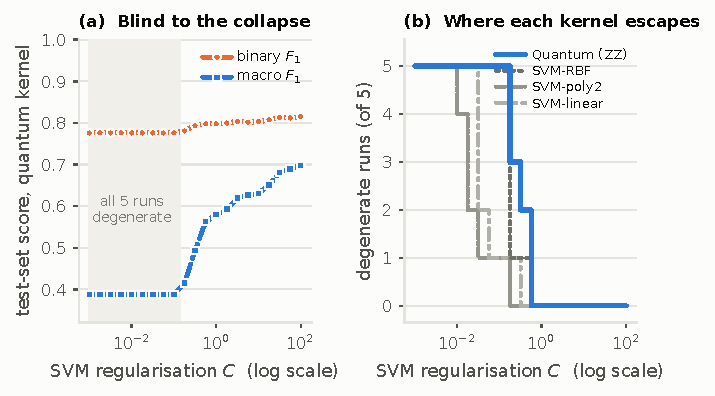
\includegraphics[width=\textwidth]{figs/fig3_objective.pdf}
  \caption{(a) The quantum kernel across the collapse boundary, on the test
  set, averaged over \pcurveRuns{} runs. Inside the shaded band every run
  predicts the attack class for all test records. Binary $\Fone$ moves by
  \pcurveFoneRise{} across the band edge; macro $\Fone$ moves by
  \pcurveMacroRise. (b) Degenerate runs against $C$ for all four kernels.
  The quantum kernel escapes between $0.1$ and $1$, where the original grid
  had no point.}
  \label{fig:objective}
\end{figure}

\paragraph{Binary $\Fone$ barely registers the collapse.}
From the degenerate band to the smallest $C$ at which no run collapses,
$C = \pcurveEscapeC$ (Fig.~\ref{fig:objective}(a)), the classifier stops
predicting a single class. Binary $\Fone$ records this as \pcurveFoneRise{}
(\pcurveFoneLo{} to \pcurveFoneHi); macro $\Fone$ as \pcurveMacroRise{}
(\pcurveMacroLo{} to \pcurveMacroHi), about \pcurveRiseRatio{} times larger.
A number that moves a little looks like a number that is working.

% Sinh boi runners/make_paper3_tables.py -- dung sua tay.
\begin{table}[t]
\centering
\caption{What selection returns on a denser grid under three
objectives, with $C$ selected once on run~1 and applied to all five
runs, as in the tuned protocol. CV score is the mean of the five
per-fold scores. \emph{Degen.} counts the runs on which the selected
model predicts the attack class for every test record. On this grid
even binary $F_1$ finds a non-degenerate $C$ for the quantum kernel,
while for the linear kernel every objective returns a $C$ that is
degenerate on one run.}
\label{tab:objective}
\begin{tabular}{l@{\hskip 1.0em}l@{\hskip 1.4em}r@{\hskip 1.4em}r@{\hskip 1.4em}r@{\hskip 1.4em}r}
\toprule
Kernel & Selection objective & Returns $C$ & CV score & Degen. & Macro $\Fone$ \\
\midrule
Quantum (ZZ) & binary $F_1$ & 0.562 & 0.8692 & 0/5 & 0.5627 \\
 & macro $F_1$ & 10 & 0.6744 & 0/5 & 0.6308 \\
 & balanced accuracy & 10 & 0.6762 & 0/5 & 0.6308 \\
\addlinespace[2pt]
SVM-RBF & binary $F_1$ & 0.316 & 0.8813 & 1/5 & 0.5422 \\
 & macro $F_1$ & 31.6 & 0.6317 & 0/5 & 0.6334 \\
 & balanced accuracy & 31.6 & 0.6333 & 0/5 & 0.6334 \\
\addlinespace[2pt]
SVM-poly2 & binary $F_1$ & 17.8 & 0.8870 & 0/5 & 0.6285 \\
 & macro $F_1$ & 17.8 & 0.6423 & 0/5 & 0.6285 \\
 & balanced accuracy & 17.8 & 0.6400 & 0/5 & 0.6285 \\
\addlinespace[2pt]
SVM-linear & binary $F_1$ & 0.0562 & 0.8813 & 1/5 & 0.5669 \\
 & macro $F_1$ & 0.0562 & 0.6216 & 1/5 & 0.5669 \\
 & balanced accuracy & 0.0562 & 0.6200 & 1/5 & 0.5669 \\
\bottomrule
\end{tabular}
\end{table}


\paragraph{The grid mattered as much as the objective.}
On the denser grid (Table~\ref{tab:objective}) every objective returns a
non-degenerate $C$ for the quantum kernel, including binary $\Fone$, which
returns $C = \pobjQBinC$ with \pobjQBinDeg{} runs degenerate: this kernel
escapes between $0.1$ and $1$, and the original grid stepped across that
interval. For the linear kernel, by contrast, all three objectives return
$C = \pobjLinBinC$, which is degenerate on \pobjLinMacDeg{} runs once it is
transferred from run~1; on the RBF kernel binary $\Fone$ is degenerate on
\pobjRbfBinDeg{} runs while both class-averaged objectives return
$C = \pobjRbfMacC$ with \pobjRbfMacDeg.

% Sinh boi runners/make_paper3_tables.py -- dung sua tay.
\begin{table}[t]
\centering
\caption{Degenerate runs (of five) when $C$ is selected separately
on each run's own training split, on the original grid, with
$N = N_{\text{train}} = N_{\text{test}}$. Q, L, P, R
are the quantum, linear, degree-two polynomial and RBF kernels. At
$N = 500$ the $\arg\max$ trap disappears, while the one-SE rule and
class weighting can still return a constant classifier.}
\label{tab:remedies}
\setlength{\tabcolsep}{3.2pt}
\begin{tabular}{lcccccccc}
\toprule
 & \multicolumn{4}{c}{$N = 100$} & \multicolumn{4}{c}{$N = 500$} \\
\cmidrule(lr){2-5}\cmidrule(lr){6-9}
Selection & Q & L & P & R & Q & L & P & R \\
\midrule
binary $F_1$, $\arg\max$ & 2 & 1 & 1 & 1 & 0 & 0 & 0 & 0 \\
binary $F_1$, one-SE rule & 2 & 1 & 1 & 1 & 0 & 1 & 2 & 0 \\
binary $F_1$, balanced class weights & 0 & 0 & 0 & 0 & 1 & 0 & 0 & 0 \\
binary $F_1$, normal class positive & 0 & 0 & 0 & 0 & 0 & 0 & 0 & 0 \\
macro $F_1$, $\arg\max$ & 0 & 0 & 0 & 0 & 0 & 0 & 0 & 0 \\
MCC, $\arg\max$ & 0 & 0 & 0 & 0 & 0 & 0 & 0 & 0 \\
\bottomrule
\end{tabular}
\end{table}


\paragraph{Per-run selection, other remedies and a larger sample.}
Table~\ref{tab:remedies} repeats the selection separately on each run's own
training split, on the original grid, at the original size and on five new
runs with $N_{\text{train}} = N_{\text{test}} = \pnLarge$ drawn by the same
sampler, which reproduces the original runs exactly. Three results stand out.
First, the three objectives in Table~\ref{tab:remedies} that read the
negative class --- macro $\Fone$, MCC, and binary $\Fone$ with the normal
class positive, whose constant baseline is $0$ --- avoided collapse in every
per-run selection, unlike the transferred selections of
Table~\ref{tab:objective}. Second, at $N = \pnLarge$ the
$\arg\max$ trap disappears for every kernel: the constant baseline is still
\pnFiveBaseline, but on every run $\arg\max$ now finds a $C$ that scores
above it and is non-degenerate on the test split, and the test macro $\Fone$ of
the selected models rises from \pmacroHundredLo--\pmacroHundredHi{} to
\pmacroFiveLo--\pmacroFiveHi, so the trap weakens once models carry real
signal. Third, two common remedies are not guarantees. The one-SE rule, which
prefers the smallest $C$ within one standard error of the best and so leans
towards collapse, returns a degenerate model at $N = \pnLarge$ for the linear
(\pprOneSeLinFive) and polynomial (\pprOneSePolyFive) kernels, and balanced
class weights do so once for the quantum kernel (\pprBalQFive). Breaking ties
towards the larger $C$ instead changed no count. What separates every
collapsed selection from the rest is a number no aggregate score displays:
the count of predicted negatives.

\section{The checks}\label{sec:checks}

The fifth contribution is a set of checks. The first recomputes every number in the text from stored
artifacts: numbers reach the prose only through generated macros, and a scan
fails the build if a literal decimal appears in a sentence. The second asserts
the invariants the argument rests on --- for example, that on the original
grid the quantum kernel's best non-degenerate score lies below the constant
baseline while each classical kernel's lies above it --- so that a regenerated
artifact that breaks the argument fails loudly. The third scans for degeneracy
over every model and all \prevRowsScanned{} rows of the revision protocol, not
only where it was expected. Each new measurement also refuses to run unless it
first reproduces the published numbers from the same code path.
Operationally, two lines in a reporting routine suffice: record the confusion
matrix beside the score, and assert that each fitted model predicts both
classes before any downstream result is computed.

\section{Limitations}\label{sec:limits}

The case comes from one corpus, one model family and four qubits.
Section~\ref{sec:catch} adds runs of \pnLarge{} records, still small by
intrusion-detection standards; the case has not been repeated under the
\prevQubits-qubit revision protocol, whose symmetric tuning was adopted partly
in response to it. The census counts runs rather than estimating a rate. With
attacks as both the majority and the positive class, binary $\Fone$ has a
high constant baseline; with the minority class positive that baseline is $0$
(Table~\ref{tab:remedies}), so this particular trap depends on that choice,
while the transfer of $C$ across sample sizes does not: the revision
protocol's collapse arose under macro $\Fone$. We
do not claim the trap is common in the literature, only that it is easy to
fall into and invisible in aggregate scores.

\section{Conclusion}\label{sec:conclusion}

Selecting $C$ by cross-validated binary $\Fone$ returned a constant
classifier whose downstream numbers looked like findings. The constant baseline
and the best genuine score differed by less than fold noise, the coarse grid
hid the escape, and a $C$ chosen on one run was reused on all. The kernel did
not cause the collapse, but its scale decided where on the $C$ axis it lay.
Objectives that read the negative class avoided it when $C$ was selected on
the run it was used for, but not always when $C$ was transferred; a denser grid,
class weighting and the one-SE rule did not always avoid it. The one
check that caught every case is also the cheapest: report the confusion
matrix beside the score.

\subsubsection*{Reproducibility.}

  All artifacts, figure scripts and audit checks are available at
  \url{https://github.com/anhquan1111/aicon2026-tuning-trap}.

\begin{thebibliography}{22}

\bibitem{companion}

Pham, M.T., Do, P.H., Nguyen, N.H.V., Nguyen, Q.A., Vo, Q.T.A.: Regime-dependent
  performance of a four-qubit quantum kernel support vector machine for network
  intrusion detection: an empirical benchmark on NSL-KDD and UNSW-NB15.
  Manuscript (2026)

\bibitem{havlicek2019}
Havl\'i\v{c}ek, V., C\'orcoles, A.D., Temme, K., Harrow, A.W., Kandala, A.,
  Chow, J.M., Gambetta, J.M.: Supervised learning with quantum-enhanced
  feature spaces. Nature \textbf{567}(7747), 209--212 (2019)

\bibitem{schuld2019hilbert}
Schuld, M., Killoran, N.: Quantum machine learning in feature Hilbert spaces.
  Phys. Rev. Lett. \textbf{122}(4), 040504 (2019)

\bibitem{liu2021speedup}
Liu, Y., Arunachalam, S., Temme, K.: A rigorous and robust quantum speed-up
  in supervised machine learning. Nat. Phys. \textbf{17}(9), 1013--1017
  (2021)

\bibitem{huang2021power}
Huang, H.Y., Broughton, M., Mohseni, M., Babbush, R., Boixo, S., Neven, H.,
  McClean, J.R.: Power of data in quantum machine learning. Nat. Commun.
  \textbf{12}, 2631 (2021)

\bibitem{shaydulin2022bandwidth}
Shaydulin, R., Wild, S.M.: Importance of kernel bandwidth in quantum machine
  learning. Phys. Rev. A \textbf{106}(4), 042407 (2022)

\bibitem{thanasilp2024concentration}
Thanasilp, S., Wang, S., Cerezo, M., Holmes, Z.: Exponential concentration in
  quantum kernel methods. Nat. Commun. \textbf{15}, 5200 (2024)

\bibitem{cortes1995svm}
Cortes, C., Vapnik, V.: Support-vector networks. Mach. Learn.
  \textbf{20}(3), 273--297 (1995)

\bibitem{chen2016xgboost}
Chen, T., Guestrin, C.: XGBoost: a scalable tree boosting system. In:
  Proceedings of the 22nd ACM SIGKDD International Conference on Knowledge
  Discovery and Data Mining, pp. 785--794 (2016)

\bibitem{breiman2001rf}
Breiman, L.: Random forests. Mach. Learn. \textbf{45}(1), 5--32 (2001)

\bibitem{payares2021dos}
Payares, E.D., Mart\'inez-Santos, J.C.: Quantum machine learning for
  intrusion detection of distributed denial of service attacks: a
  comparative overview. In: Quantum Computing, Communication, and Simulation.
  Proc. SPIE, vol. 11699, 116990B (2021)

\bibitem{kalinin2023qids}
Kalinin, M.O., Krundyshev, V.M.: Security intrusion detection using quantum
  machine learning techniques. J. Comput. Virol. Hacking Tech.
  \textbf{19}(1), 125--136 (2023)

\bibitem{abreu2025quantumnetsec}
Abreu, D., Moura, D., Rothenberg, C.E., Abel\'em, A.: QuantumNetSec: quantum
  machine learning for network security. Int. J. Netw. Manag.
  \textbf{35}(4), e70018 (2025)

\bibitem{kaissar2026survey}
Kaissar, A., Bou~Nassif, A., Bouridane, A.: Enhancing network intrusion
  detection with quantum machine learning: a comprehensive survey of
  methods, metrics, and applications. Future Internet \textbf{18}(5), 234
  (2026)

\bibitem{chicco2020mcc}
Chicco, D., Jurman, G.: The advantages of the Matthews correlation
  coefficient (MCC) over F1 score and accuracy in binary classification
  evaluation. BMC Genomics \textbf{21}(1), 6 (2020)

\bibitem{christen2023fmeasure}
Christen, P., Hand, D.J., Kirielle, N.: A review of the F-measure: its
  history, properties, criticism, and alternatives. ACM Comput. Surv.
  \textbf{56}(3), 73 (2023)

\bibitem{saito2015prc}
Saito, T., Rehmsmeier, M.: The precision-recall plot is more informative than
  the ROC plot when evaluating binary classifiers on imbalanced datasets.
  PLoS ONE \textbf{10}(3), e0118432 (2015)

\bibitem{he2009imbalanced}
He, H., Garcia, E.A.: Learning from imbalanced data. IEEE Trans. Knowl. Data
  Eng. \textbf{21}(9), 1263--1284 (2009)

\bibitem{forman2010apples}
Forman, G., Scholz, M.: Apples-to-apples in cross-validation studies:
  pitfalls in classifier performance measurement. ACM SIGKDD Explor. Newsl.
  \textbf{12}(1), 49--57 (2010)

\bibitem{cawley2010overfitting}
Cawley, G.C., Talbot, N.L.C.: On over-fitting in model selection and
  subsequent selection bias in performance evaluation. J. Mach. Learn. Res.
  \textbf{11}, 2079--2107 (2010)

\bibitem{arp2022mlsec}
Arp, D., Quiring, E., Pendlebury, F., Warnecke, A., Pierazzi, F.,
  Wressnegger, C., Cavallaro, L., Rieck, K.: Dos and don'ts of machine
  learning in computer security. In: 31st USENIX Security Symposium,
  pp. 3971--3988 (2022)

\bibitem{moustafa2015unsw}
Moustafa, N., Slay, J.: UNSW-NB15: a comprehensive data set for network
  intrusion detection systems. In: 2015 Military Communications and
  Information Systems Conference (MilCIS), pp. 1--6. IEEE (2015)

\end{thebibliography}

\end{document}
